\begin{frame}
	\frametitle{What is the Problem?}
	\only<1>{
		\begin{figure}
			\begin{tikzpicture}[
	scale = 0.6,
	idea/.style={
		cloud,
		draw=black,
		aspect=3
	},
	every node/.style={
		font=\footnotesize
	}
]{
		\def\width{16}
		\def\height{9}
%		\draw[help lines, opacity=0.5] (0,0) grid (\width,\height);
		\node(i1)[idea] at (8,4.5){(Autonomous) Distributed Data Processing};
}
\end{tikzpicture}
		\end{figure}
	}
	\only<2>{
		\begin{figure}
			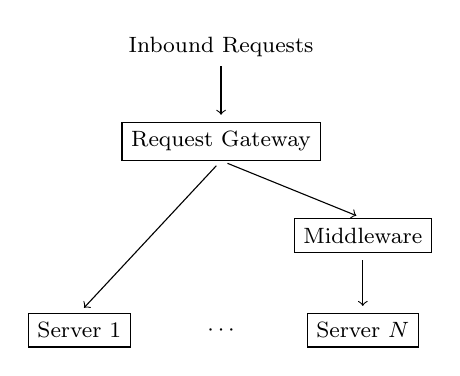
\begin{tikzpicture}[
	scale = 0.6,
	rect/.style={
		rectangle,
		draw=black
	},
	every node/.style={
		font=\footnotesize
	}
	]{
		\def\width{16}
		\def\height{9}
		%\draw[help lines, opacity=0.5] (0,0) grid (\width,\height);
		\node(p1) at (8,7) {Inbound Requests};
		\node[rect](g1) at (8,5){Request Gateway};
		\node[rect](s1) at (5,1){Server 1};
		\node(d1) at (8,1){\(\cdots\)};
		\node[rect](s2) at (11,1){Server \(N\)};
		\node[rect](s3) at (11,3){Middleware};
		
		\path[->, shorten >=0.25em] 										(p1.south) 	edge (g1.north);
		\path[->, shorten >=0.25em, shorten <=0.25em] 	(g1.south) 	edge (s1.north)
																																edge (s3.north);
		\path[->, shorten >=0.25em, shorten <=0.25em] 	(s3.south) 	edge (s2.north);																														
	}
\end{tikzpicture}
			\caption{Simple Example: Inbound requests are divided into heterogeneous data-parallel operations (with dependencies) that are %
				routed across a collection of backends.}
		\end{figure}
	}
	\only<3>{
		\Large \textbf{What have we tried?} \normalsize\vspace{1em}
		\begin{columns}
			\begin{column}{0.45\textwidth}
				\begin{itemize}
					\item MapReduce
					\item Dryad
					\item Spark
					\item Hadoop
					\item Storm
					\item and on...
					\item \footnotesize and on...
					\item \scriptsize and on...
				\end{itemize}
			\end{column}
			\begin{column}{0.45\textwidth}
				\begin{itemize}
					\item Docker
					\item Kubernetes
					\item OpenWhisk
					\item OpenFaas
					\item KNative
					\item and on...
					\item \footnotesize and on...
					\item \scriptsize and on...
				\end{itemize}
			\end{column}
		\end{columns}
	}
	\only<4>{
		\begin{center}
			\LARGE Has any of it actually worked?
		\end{center}
	}
	\only<5>{
		\begin{figure}
			\includegraphics[width=0.6\textwidth]{./figures/standards.png}
			\caption{\scriptsize Courtesy of XKCD. (\href{https://xkcd.com/927/}{https://xkcd.com/927/})}
		\end{figure}
	}
\end{frame}